\apendice{Documentación de usuario}

\section{Introducción}

En este apartado se mostrarán los requisitos necesarios para instalar la aplicación y un detallado manual en el que se explica cómo funciona la aplicación. 

\section{Requisitos de usuarios}

El usuario, para poder ejecutar la aplicación ha de poseer un equipo con sistema operativo Windows 10 y una máquina virtual con un sistema operativo Ubuntu-server.

\section{Instalación}

Los pasos para instalar la aplicación se encuentran detalladas en el anexo dedicado a la instalación y compilación dentro del manual del programador.


\section{Manual del usuario}

Este apartado pretende hacer de guía al usuario a través de la aplicación, mostrando cómo funciona el sistema y cómo es posible configurarlo.

\subsection{Configuración}

Una vez instalado el programa el usuario podrá elegir que sensores desea almacenar y entrenar así cómo elegir cada cuanto tiempo se desea ejecutar el programa y seleccionar cuantos instantes de tiempo en el futuro se desea predecir. Para ello se ha de acceder al fichero \textit{/usr/bin/Monitorizacion\_IOT/Monitorizacion\_IOT.sh} en él, se encintarán una serie de variables que el usuario ha de modificar.

\begin{itemize}
    \item \textbf{usuario\_PRTG}: se ha de introducir el nombre de usuario de PRTG
    \item \textbf{passhash\_PRTG}: se ha de introducir el passhash de PRTG
    \item \textbf{lista\_id\_sensor}: En esta lista se ha de introducir el id de los sensores, separados por un espacio.
    \item \textbf{horizonte\_predicción}: se ha de introducir cuantos minutos a futuro se desea que llegue la predicción.
    \item \textbf{tiempo\_espera}: Se ha de introducir el tiempo en segundos que ha de esperar el sistema entre ciclo y ciclo. 
\end{itemize}

\subsection{Inicialización y parada del sistema}

Una vez configurado el programa se puede inicializar y poner en marcha todo el sistema, para ello se ha de introducir el siguiente comando:

\begin{lstlisting}[frame=single]  
systemctl start Monitorizacion_IOT
\end{lstlisting}

para realizar la parada completa del sistema y que este deje de captar datos de PRTG se ha de introducir el siguiente comando:

\begin{lstlisting}[frame=single]  
systemctl stop Monitorizacion_IOT
\end{lstlisting}

\subsection{Obtención y almacenamiento de datos}\label{cap:obt_alm_datos}

Para poder trabajar con los datos de los sensores inicialmente almacenados en PRTG era necesario descargarlos y almacenarlos por nuestra cuenta, para poder realizar el estudio y entrenamiento de dichos datos.

\nombrePrograma mediante un script descarga los datos de los sensores que se encuentran en la lista \textbf{lista\_id\_sensor}, estos se guardan en un fichero JSON, el cual hay que transformar para adecuar el formato del fichero y que Elasticsearch pueda procesarlo. Para almacenar los datos ya obtenidos y transformados a la base de datos de Elasticsearch, estos ficheros son preprocesados por logstash que se encarga de enviar las líneas de datos al servidor de Elastic e indexarlos correctamente.

Los datos son subidos con el siguiente nombre: ``sensor\_data-yyyy.mm.dd'' de tal forma que todos los datos que se almacenan en un día se almacenan bajo un mismo índice. Para poder explorar y visualizar los datos en Kibana es necesarios que exista un ``index pattern'' que diga a Elasticsearch que índices contienen los datos así como especificar de que tipo son, en este caso se ha creado uno para que albergue todo los datos procedentes de sensores ``sensor\_data-*''. 

Una vez los datos estén correctamente almacenados e indexados en Elasticsearch, podemos proceder a explorar y visualizar los datos con Kibana.

Elasticsearch provee un motor de búsqueda utilizando Query DSL (lenguaje de dominio específico) lo que nos permite filtrar fácilmente entre todos los datos que se van almacenando.

\begin{figure}[h]
	\centering
	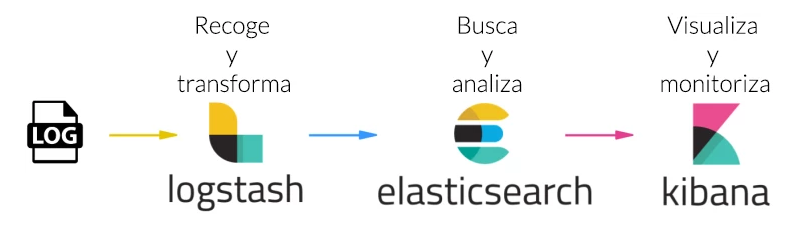
\includegraphics[width=1.1\textwidth]{img/img_resumen_ELK.png}
	\caption{ELK stack}
	\label{img_Consumo_Bomba_Agua}
\end{figure}

\subsubsection{Transformación de datos}\label{cap:TransformacionDatos}


Para la transformación del fichero JSON, se empiezo utilizando un sencillo programa en Flex, un procesador de lenguaje, que eliminaba los datos irrelevantes que se obtenían de PRTG y añadía el id del sensor, así como separaba las líneas dentro del fichero para poder mandárselo a Elasticsearch a través de logstash cómo campo el ID del sensor, cómo se puede observar el los Listings \ref{json-example} y \ref{json-transformado-example}

Tras un tiempo y debido a que era necesario modificar el formato de las fechas se decidió pasar esta funcionalidad a Python ya que facilita el tratamiento con fechas.


\begin{listing}
\begin{minted}[frame=single,
               framesep=3mm,
               linenos=true,
               xleftmargin=21pt,
               tabsize=6]{js}
{
    "prtg-version":"21.2.68.1492",
    "treesize":30,
    "histdata":
    [
        {
            "datetime":"27/07/2021 16:11:06",
            "Valor":4.6800,
            "Tiempo de ejecución":782.0000,
            "coverage":"100 %"
        },
        {
            "datetime":"27/07/2021 16:12:06",
            "Valor":4.6800,
            "Tiempo de ejecución":797.0000,
            "coverage":"100 %"
        },
        {
            "datetime":"27/07/2021 16:13:06",
            "Valor":4.6700,
            "Tiempo de ejecución":799.0000,
            "coverage":"100 %"
        }
    ]
}

\end{minted}
\caption{JSON descargado de PRTG} 
\label{json-example}
\end{listing}

\begin{listing}
\begin{minted}[frame=single,
               framesep=3mm,
               linenos=true,
               xleftmargin=21pt,
               tabsize=6]{js}

{
    "sensorId":"2051",
    "datetime":"27/07/2021 16:11:06",
    "reading": 
    {
        "Valor":4.6800,
        "Tiempo de ejecución":782.0000
    }
}
{
    "sensorId":"2051",
    "datetime":"27/07/2021 16:12:06",
    "reading": 
    {
        "Valor":4.6800,
        "Tiempo de ejecución":797.0000
    }
}
{
    "sensorId":"2051",
    "datetime":"27/07/2021 16:13:06",
    "reading": 
    {
        "Valor":4.6700,
        "Tiempo de ejecución":799.0000
    }
}

\end{minted}
\caption{JSON transformado} 
\label{json-transformado-example}
\end{listing}

\newpage
\begin{comment}
\section{Diseño del proyecto}

El núcleo del programa es el script \textit{Monitorizacion_IOT} el cual es un servicio que se repite cada X segundos.

\noindent\fbox{
\begin{minipage}{1\textwidth}
\begin{algorithmic}[1]

\While{True}
    
    \For{id in listaSensores}
        \State $fechaInicio \gets Fecha del sistema - 30 minutos$
        \State $fechaFin \gets Fecha del sistema $
        
        \If{fichero ""tempData"" + id + "".json"" exist}
            \State descarga\_datos\_PRTG
            \State transformar\_datos
            \State comparar\_ficheros
            \State subir\_datos
            
            \State Copiar
            \State Borrar
        \Else
            \State descarga\_datos\_PRTG
            \State transformar\_datos
            \State subir\_datos
            
            \State Copiar
            \State Borrar
        \EndIf
        
        \State Entrenar Modelo
        \State Subir Datos entrenamiento
        
        \State Borrar\_datos\_predicciones
        \State Predecir
        \State Subir datos predicción
        
    \EndFor
\EndWhile

\end{algorithmic}
\end{minipage}
}
\end{comment}
\section{Machine learning}

\subsubsection{Incremental/Online Learning}

Cómo se ha especificado en apartado de conceptos teóricos el incremental learning va entrenando el modelo con datos en un flujo continuo. 

En nuestro caso esto es muy beneficioso ya que no disponemos de muestras lo suficientemente grandes como para entrenar un modelo de forma eficaz. 

por lo que el modelo va aprendiendo a medida que se van recogiendo los datos, esto hace a nuestro algoritmo sea escalable.

\subsection{Modelos}

La librería de Python, River, nos facilita dos tipos de modelos para series temporales que nos permitirán realizar el entrenamiento de manera incremental con un data stream procedente de nuestros sensores así cómo realizar una predicción del comportamiento de nuestros sensores.

Pese a que solo estén implementados en la aplicación dos tipos de modelos la aplicación está preparada para que se pueda implementar nuevos tipos de modelos de diversas librerías.

Antes de nada, se ha de crear un modelo para un id en concreto, se puede decidir qué tipo de modelo así cómo los parámetros necesarios.

\subsection{Crear un modelo para un sensor}

para crear un modelo para un sensor hay que modificar de forma manual el fichero /usr/bin/Monitorizacion-IOT/Prediccion/Crear\_modelo.py una vez en el fichero se ha de generar una instancia del modelo que se dese crear pasando cómo parámetro el id del sensor. A continuación, llamaremos a la función inicializar de nuestro modelo, pasándole los parámetros necesarios. Para guardar el modelo simplemente compilamos el fichero, este se guardará en la carpeta /usr/bin/Monitorizacion-IOT/Prediccion/modelos/ y se podrá usar para el entrenamiento y la predicción.

\begin{verbatim}
if __name__ == "__main__":

    idSensor = 4051

    modelo = Modelo_SNARIMAX(idSensor)
    modelo.inicializar(q=2,
                        m=30,
                        sp=6,
                        sq=10,
                        intercept_init=12,
                        sgd=0.01, 
                        intercerpt_lr=0.3)

    Persistencia_modelo.guardar(modelo)

\end{verbatim}
\begin{comment}
\subsubsection{Detrender}
El modelo Detrender se caracteriza por eliminar tendencias en series de tiempo, 
centra el target u objetivo en 0 

\begin{verbatim}
    def _inicializar(self):

        extract_features = compose.TransformerUnion(Modelo._get_ordinal_date)

        scale = preprocessing.StandardScaler()

        learn = linear_model.LinearRegression(
            intercept_lr=self.intercept_lr,
            optimizer=optim.SGD(self.sgd)
        )

        model = extract_features | scale | learn

        model = time_series.Detrender(regressor=model, window_size=self.window)


        return model
\end{verbatim}

\subsubsection{SNARIMAX}

SNARIMAX por sus siglas (S)easonal (N)on-linear (A)uto(R)egressive (I)ntegrated (M)oving-(A)verage with e(X)ogenous.

Este modelo asume que los datos de entrenamiento recibidos están ordenados por tiempo y espaciados uniformemente.

Componentes:
\begin{itemize}
    \item \textbf{Seasonal - Non-linear}: No es necesario utilizar una regresión lineal, se puede utilizar cualquier tipo de regresión.
    \item \textbf{Autoregredive}:
    \item \textbf{Integrated}:
    \item \textbf{Moving-Avarage}:
    \item \textbf{Exogenous}: Se pueden implementar funciones adicionales.
\end{itemize}

Estos componentes se pueden activar o desactivar a la hora de crear el modelo.

Parámetros:
\begin{itemize}
    \item \textbf{p}:
    \item \textbf{d}:
    \item \textbf{q}:
    \item \textbf{m}:
    \item \textbf{sp}:
    \item \textbf{sd}:
    \item \textbf{pq}:
    \item \textbf{regressor}:
\end{itemize}

\begin{verbatim}
   def _inicializar(self):

        extract_features = compose.TransformerUnion(
            Modelo._get_ordinal_date,
        )

        model = (
            extract_features |
            time_series.SNARIMAX(
                p=self.p,
                d=self.d,
                q=self.q,
                m=self.m,
                sp=self.sp,
                sq=self.sq,
                regressor=(
                    preprocessing.StandardScaler() |
                    linear_model.LinearRegression(
                        intercept_init= self.intercept_init,
                        optimizer=optim.SGD(self.sgd),
                        intercept_lr= self.intercerpt_lr
                    )
                )
            )
        )

        return model
\end{verbatim}
\end{comment}
\subsection{Entrenamiento}

Una vez los datos procedentes de los sensores han sido correctamente se puede realizar el entrenamiento de los modelos.

Por cada sensor que se dese entrenar se cargará el modelo que se haya creado para ese modelo en concreto y se descargarán los datos en un rango de fecha determinado desde Elasticsearch.

los valores de entrenamiento serán volcados a un fichero y devueltos a Elasticsearch.

Una vez acabado el entrenamiento se guarda el modelo en disco para que la siguiente vez que se requiera entrenar modelo o hacer predicciones se utilice siempre el modelo más actualizado.


\subsection{Predicción}

Cada ciclo del programa se hace una predicción de los siguientes minutos, para no acumular datos repetidos en la BBDD se eliminan los datos que se han predicho en el ciclo anterior Así cada predicción que hace el programa esta actualizada y utiliza el modelo más entrenado disponible.

Para ello cada vez que se hace la perdición se carga el modelo que se ha entrenado para un sensor específico y se le pide que saque una predicción de los instantes de tiempo que se especifiquen

\begin{figure}[h]
	\centering
	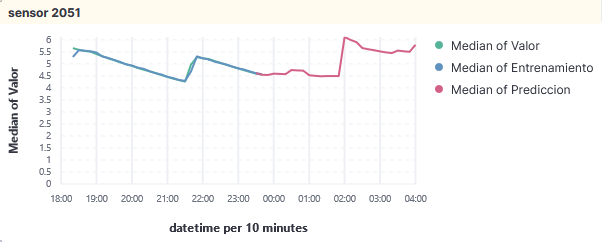
\includegraphics[width=1.1\textwidth]{img/img_prediccion_sensor2051.png}
	\caption{predicción sensor de Presión Tubería de Agua}
	\label{img_prediccion_sensor2051}
\end{figure}


\section{Visualización y monitorización}

Para poder visualizar y monitorizar nuestros datos debe de estar nuestro servidor funcionando.

Mediante un navegador introducimos la siguiente url: IP\_ubuntu\_server:5601 el puerto 5601 corresponde al de kibana.

\begin{figure}[h]
	\centering
	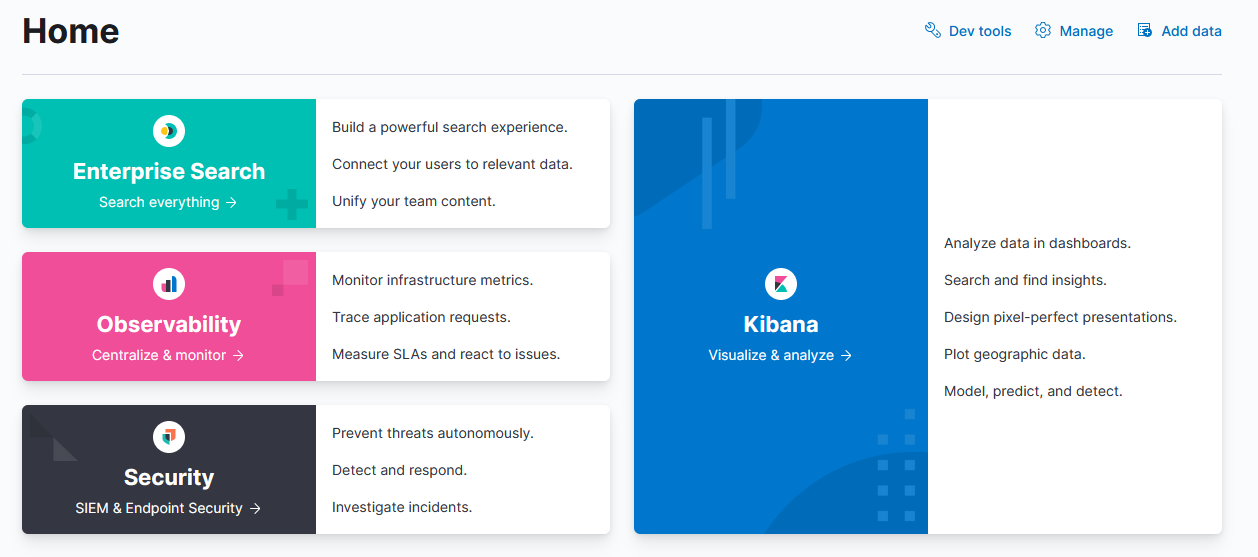
\includegraphics[width=1.1\textwidth]{img/img_kibana_home.png}
	\caption{pagina inicio kibana}
	\label{img_kibana_home}
\end{figure}

Una vez en el apartado home podemos acceder al apartado ``kibana Visualize & analyze'' para poder echar un vistazo a nuestros datos. Para ver ver nuestros datos, así como realizar filtrados y búsquedas accederemos a ``Discover''

Se pueden visualizar los datos que estén vinculados a un patrón de índices.

\begin{figure}[h]
	\centering
	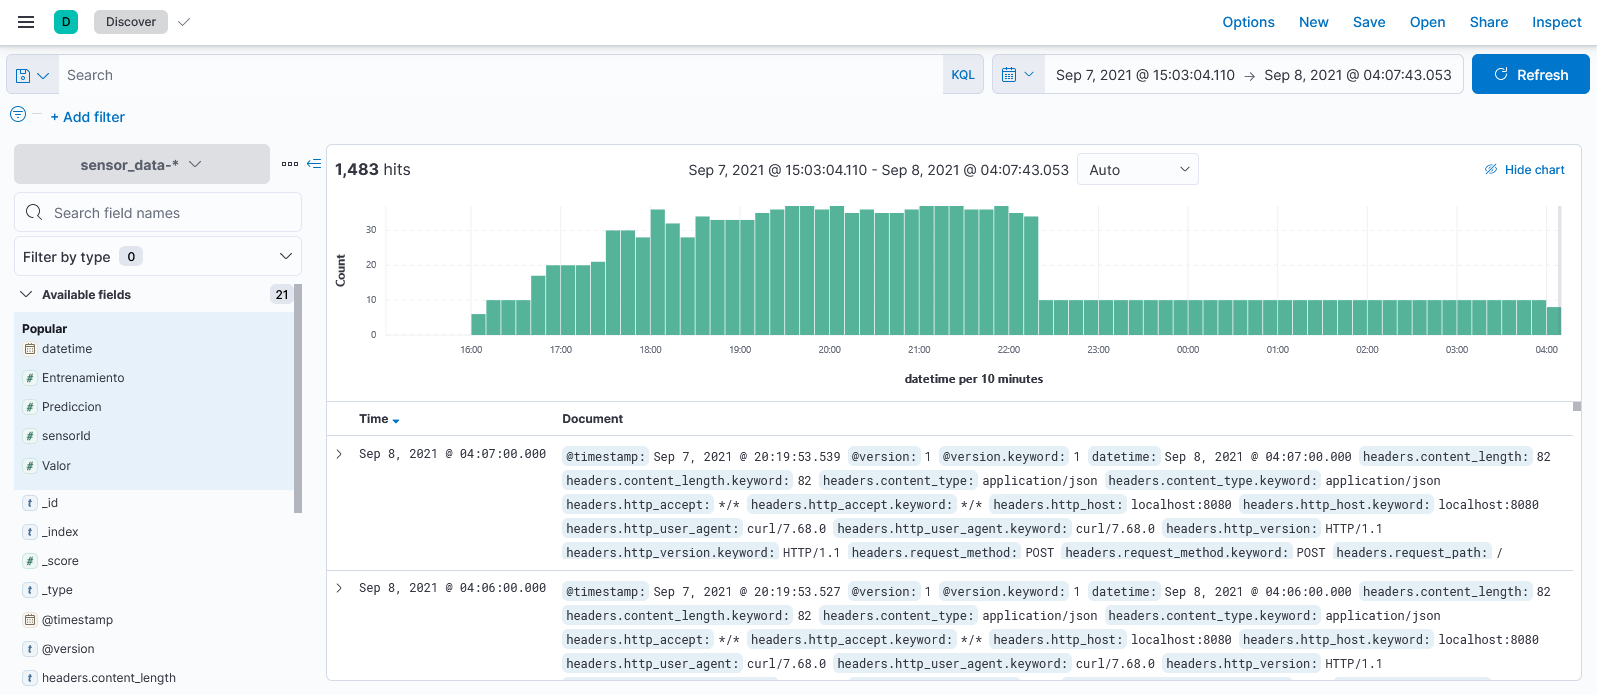
\includegraphics[width=1.1\textwidth]{img/img_kibana_discover.png}
	\caption{kibana discover}
	\label{img_kibana_discover}
\end{figure}

Para visualizar de forma gráfica nuestros datos accederemos al apartado ``Dashboard'' en el podemos crear cualquier tipo de gráfico.

\begin{figure}[h]
	\centering
	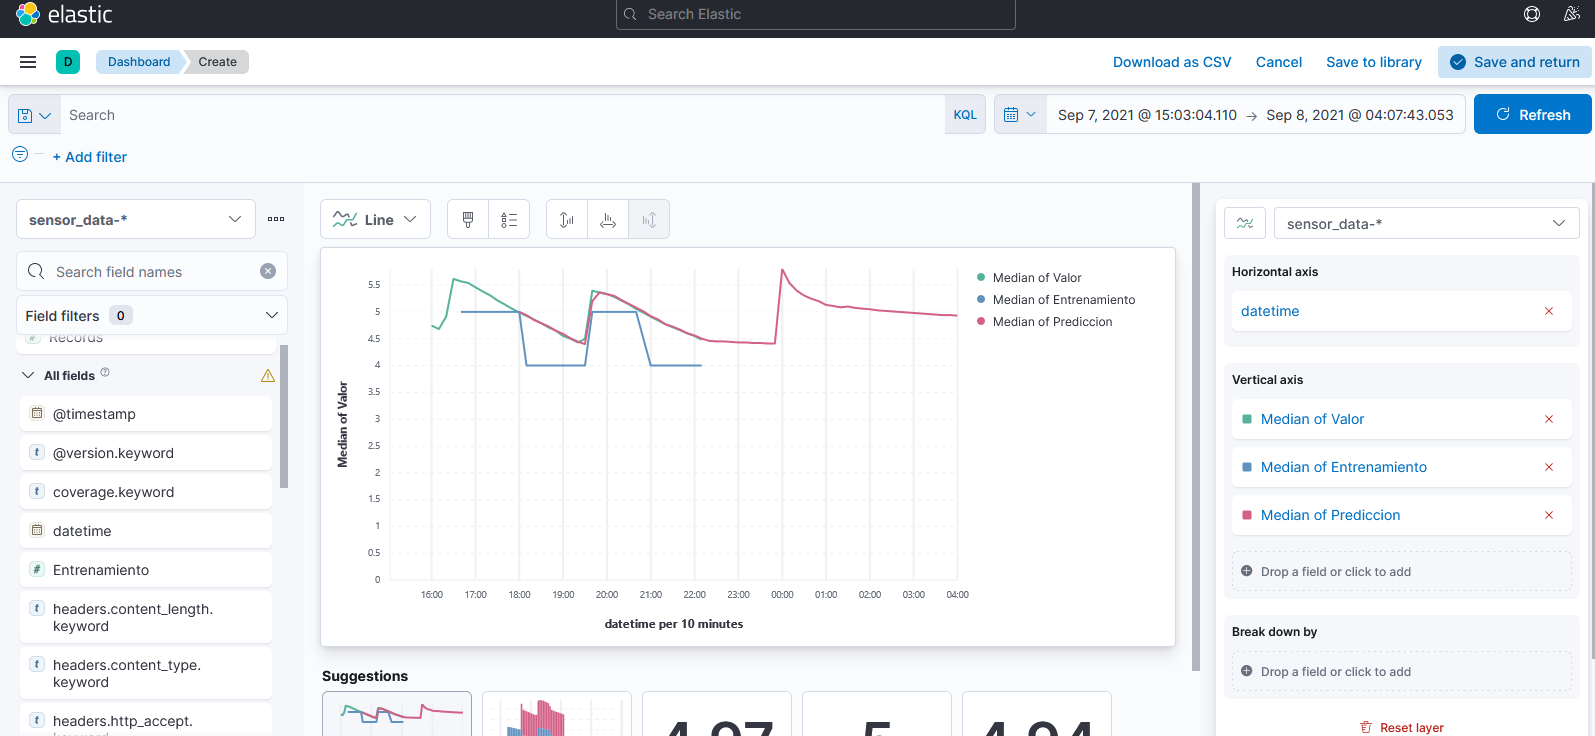
\includegraphics[width=1.1\textwidth]{img/img_kibana_dashboard.png}
	\caption{kibana dashboard}
	\label{img_kibana_dashboard}
\end{figure}

Para más información acceder a la documentación de kibana en el que se detalla todo lo que se puede realizar con esta herramienta de visualización.


